\chapter{Maximum independent set problem}
\section{Purpose of study}
Optimization has been expanding in all directions at an astonishing rate during
the last decades. New algorithmic and theoretical techniques have been developed,
the diffusion into other disciplines has proceeded at a rapid pace, and our knowledge
of all aspects of the field has grown even more profound. At the same time,
one of the most striking trends in optimization is the constantly increasing emphasis on the interdisciplinary nature of the field. Optimization today is
basic research
tool in all areas of engineering, medicine and the sciences. The decision making tools
based on optimization procedures are successfully applied in a wide range of practical
problems arising in virtually any sphere of human activities, including biomedicine,
energy management, aerospace research, telecommunications and finance.

Practical applications of the considered optimization problems are abundant.
They appear in information retrieval, signal transmission analysis, classification
theory, economics, scheduling, experimental design, and computer vision. Among the known problems 
that come down to finding an independent set are the following: 
matching molecular structure \cite{molecular_matching}, 
macromolecular docking \cite{molecular_docking},
integration of genome mapping data \cite{genome_mapping}, 
comparative modeling of protein structure\cite{modeling_protein_structure}, covering location using clique partition \cite{butenko_applications} etc.

Considering the theoretical significance and practical relevance of the MCP, a lot of time and attention has been put into developing different solution methods. On the one hand, the generic branch-and-bound (B\&B) framework has served as the foundation for several useful accurate approaches. These techniques offer the potential benefit of ensuring that the answer found is the best one possible. However, due to the MCP's intrinsic computational complexity, accurate techniques sometimes only work for small issues and can be computationally expensive in general. On the other hand, several heuristic and metaheuristic algorithms have been developed with the aim of delivering sub-optimal solutions to huge problems that can't be solved optimally in a reasonable amount of time.

A lot of real life problems use graph theory and converge to maximum clique problem. Finding the maximum clique $MC$ in the graph $G$ is $NP$-hard problem and is the same as finding maximum independent set $MIS$ on the complementary graph $G'$. 

\section{Problem definition}
Given an undirected graph \graphG where $V$ - finite set of vertices and $E$ - finite set of edges.

\newtheorem{definition}{Definition}[section]
\begin{definition} [Complement graph]
Complement graph $G'=(V,E')$ is a graph s.t. for $\forall e\in E' \iff e\notin E$ 
\end{definition}
\begin{definition} [Clique]
Clique $C$ in an undirected graph \graphG is a subset of vertices $C\subseteq V$ such that every two distinct vertices are adjacent. This is equivalent to the condition that the induced subgraph of G induced by C is a complete graph.
\end{definition}
\begin{definition} [Maximal clique]
Maximal clique $MaxC$ is a clique that cannot be extended by including one more adjacent vertex, that is, a clique which does not exist exclusively within the vertex set of a larger clique.
\end{definition}
\begin{definition} [Maximum clique]
Maximum clique $MC$ of a graph \graphG is a clique, such that there is no clique with more vertices. Moreover, the clique number $\omega(G)$ of a graph $G$ is the number of vertices in a maximum clique in $G$.
\end{definition}
\begin{definition}[Independent set]
Independent set in graph \graphG is a set of vertices $S \subseteq V$ such that no vertices in $S$ are adjacent to each other.
\end{definition}

For a subset $U$ of vertices $V$ of graph \graphG $U \subseteq V$, $G[U] = (U,E[U])$ is used to represent the subgraph \textbf{induced} by $U$, s.t. edges of $U$ is a set $E[U] = \{(u,v)\in E | u,v\in U\}$

\begin{figure}[h]
    \centering
    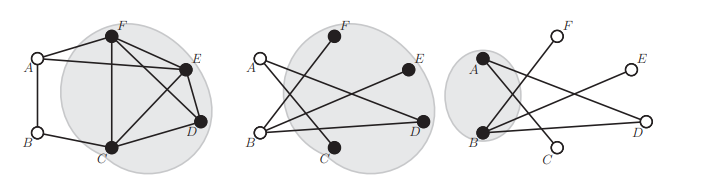
\includegraphics{figures/graph_clique_IS_dependencies.png}
    \caption{An illustration of the relation between maximum clique, maximum independent set and minimum vertex cover. Given the initial graph $G$ with $V = \{A, B, C,D, E, F\}$(left) and its complementary graph $G$ (middle/right), the set of vertices $\{C,D, E, F\}$ is a maximum clique of $G$ and an maximum independent set of $G$ while ${A, B} = V \ {C,D, E, F}$ is a minimum vertex cover of $G$}
    \label{fig:graph_clique_IS_dependencies}
\end{figure}

\begin{definition}[Maximum independent set problem]
The Maximum Independent Set \textit{MIS} problem in graph theory is the task of finding
the largest independent set in a graph.
\end{definition}

There are many research on the MIS formulation. These investigations hold a great deal of interest since they have the potential to deepen our understanding of the issue at hand and yield novel theoretical and applied findings.
The following binary problem gives the simplest formulation:
\begin{subequations} \label{mis_binary_formulation_1}
\begin{equation} 
    \text{maximize} \sum_{i=1}^n x_i
\end{equation}
\begin{equation}
    \text{subject to } x_i+x_j \leq 1, \forall \{i,j\}\in E
\end{equation}
\begin{equation}
    x_i \in \{0,1\}, i = 1,...,n
\end{equation}
\end{subequations}

An alternative formulation of this problem is the following \textit{clique formulation}:
\begin{subequations}\label{clique_binary_formulation_1}
\begin{equation}
    \text{maximize} \sum_{i=1}^n x_i
\end{equation}
\begin{equation} \label{clique_binary_formulation_2}
    \text{subject to } x_i \leq 1, \forall S \in C \equiv \text{\{maximal cliques of $G$\}}
\end{equation}
\begin{equation}
    x_i \in \{0,1\}, i = 1,...,n
\end{equation}
\end{subequations}

The advantage of formulation \ref{clique_binary_formulation_1} over \ref{mis_binary_formulation_1} is a smaller gap between the optimal
values of \ref{clique_binary_formulation_1} and its linear relaxation, however
 finding a good solution to \ref{clique_binary_formulation_1} is challenging since the number of restrictions in \ref{clique_binary_formulation_2} is exponential.

 Here we mention one more integer programming formulation. Let $A_G$ be the
adjacency matrix of a graph \graphG, and let $J$ denote the $nxn$ identity matrix. The
maximum independent set problem is equivalent to the global quadratic zero-one problem
\begin{subequations} \label{mis_matrix_furmulation}
\begin{equation}
    \max f(x) = x^TAx   
\end{equation}
subject to 
\begin{equation}
    x_i \in \{0,1\}, i = 1,...,n
\end{equation}
\end{subequations}
where $A = J - A_G$. If $x^*$ is a solution to \ref{mis_matrix_furmulation}, then the set $\mathcal{I}$ defined by $\mathcal{I}=\{i\in V:{x_i}^*=1\}$ is the MIS of $G$ with $|\mathcal{I}|=f(x^*)$.

The independent set problem and the clique problem are complementary: a clique in \graphG is an independent set in the complement graph of $G$ and vice versa. Therefore, many computational results may be applied equally well to either problem. For example, the results related to the clique problem have the following corollaries:

\begin{itemize}
    \item The independent set decision problem is $NP$-complete, and hence it is not believed that there is an efficient algorithm for solving it.
    \item The maximum independent set problem is $NP$-hard and it is also hard to approximate.
\end{itemize}

Despite the close relationship between maximum cliques and maximum independent sets in arbitrary graphs, the independent set and clique problems may be very different when restricted to special classes of graphs. For instance, for sparse graphs (graphs in which the number of edges is at most a constant times the number of vertices in any subgraph), the maximum clique has bounded size and may be found exactly in linear time.

There is currently no known efficient algorithm to find maximum independent sets, however there are powerful heuristic algorithms to solve this problem like ReduMIS \cite{redumis}, IBM CPLEX LP-solver \cite{CPLEX}, branch-reduce algorithms and others. The most recent state-of-art solver ReduMIS uses iterative implementation of a series of graph reduction techniques and evolutionary algorithm. CPLEX uses plain integer linear programming solving to obtain the solution. Despite these algorithms return quite accurate results they have large disadvantage - they are very time consuming and not appropriate for large graphs regarding memory consumption. 
The main idea of improvement is to use algorithm that can obtain solution in more parallelized way using neural networks.

\section{Heuristics for MIS problem}
Even on graphs with several hundred vertices, exact approaches become impractical (too slow) despite providing the best solution. Because of this such approaches cannot be used to solve the maximum independent set problem on very large graphs, thus heuristic solutions are the ones that can be used.
Perhaps the most straightforward heuristics for the maximum independent set problem are sequential greedy heuristics, which repeatedly add a vertex to an intermediate independent set ("Best in") or remove a vertex from a set of vertices that is not an independent set ("Worst out") based on some criterion, say the degrees of the vertices \cite{j74}, \cite{kr87}.
People occasionally look to nature for effective heuristics because it always seems to have the best answers. New types of optimization algorithms that essentially try to mimic specific natural processes have recently been created and successfully tested.

The design of simulated annealing \cite{kgv83}, neural networks \cite{h82}, and evolutionary computation \cite{h75} methods in the field of optimization were influenced by the natural phenomenal observed in annealing processes, nervous systems, and natural evolution. Other well-liked metaheuristics are tabu search \cite{gl97} and greedy randomized adaptive search procedures, or GRASP \cite{fr95}. These heuristics have been successfully used in various forms to solve numerous significant combinatorial optimization issues, including the maximum independent set problem. Below, we'll quickly go over a few of these heuristics.

\subsection{Greedy randomized algorithm}
An iterative randomized sampling technique called a greedy randomized adaptive search procedure (GRASP) provides a heuristic solution to the current problem with each iteration \cite{fr95} in a subtle way. The final outcome for all intents and purposes is literally the best solution across all GRASP iterations. Each GRASP iteration consists of two phases: the first creates a restricted candidate list (RCL) of solutions using an adaptive randomized greedy function; the second one attempts to find an improvement by using a local search technique. 
The so-called path relinking \cite{glm00} , a recent addition to GRASP, has been proposed to improve the performance of the heuristic by connecting good quality solutions with a path of intermediate feasible points. It seems that many of these possible places offer solutions of higher quality than the ones picked as the path's endpoints. For difficult problems with the maximal independent set or graph coloring, the GRASP approach with path relinking can be used.

The success of machine learning solutions for reasoning about discrete structures has brought attention to its adoption within combinatorial optimization algorithms. These approaches usually rely on supervised learning by leveraging datasets of the combinatorial structures of interest drawn from some distribution of problem instances. Reinforcement learning has also been employed to find such structures. We propose an approach such that no data is necessary for training the networks that produce the solution. The suggested technique is not machine learning in this sense. However, it relies on neural networks and applies backpropagation to a loss function determined by the architecture of the neural network rather than a training dataset. To handle large-scale graphs, we also suggest a general graph reduction method. The reduction, which works with any graph type and/or density, takes advantage of community detection for graph splitting. Also some postprocessing of the neural network result is included to improve the final result.

\subsection{Genetic algorithms}

Natural system evolution processes served as the inspiration for genetic algorithms in optimization. A population of points, also known as individuals or chromosomes, are used for optimization in a genetic algorithm. The chromosomes are represented in the most basic form by binary vectors. Each chromosome has a fitness value, which measures the likelihood that the person designated by that chromosome will live to adulthood in the following generation. Values of the objective function that represents the population's overall fitness are computed using individual fitness values. An optimization technique may be built on the fundamental law of natural selection, which states that population fitness as a whole doesn't decline with time.

The genetic algorithm, in its most basic form, begins with a population selected at random and computes a new population using one of three fundamental mechanisms: reproduction, crossover, or mutation \cite{g89}. According to the likelihood provided by their fitness, the reproduction operator selects the chromosomes employed in the following generation. To create additional offspring from a pair of parents and children, the crossover operator is used. Finally, the mutation operator, with a specified probability, flips the value of each bit in a chromosome.

From the beginning of the 1990s, early attempts were made to use genetic algorithms to solve the maximum independent set and maximum clique problems. Since then, several effective implementations have been documented in the literature \cite{be95}, \cite{h97}, \cite{m02}. The majority of genetic algorithms are simple to parallelize.

\subsection{Simmulated annealing}

In physics, the annealing procedure is used to create a pure lattice structure. It entails heating a solid to melt it, followed by progressively cooling it to a low-energy state to solidify it. This procedure minimizes the free energy of the system. In the simulated annealing approach, where each viable solution represents a state of the fictitious physical system and the objective function represents the energy corresponding to that state, this characteristic of the annealing process is employed for optimization purposes. The following is the fundamental idea of simulated annealing:
Generate an initial feasible solution $x^{(0)}$. On the iteration $k+1$, given a solution $x^{(k)}$, accept it's neighbours $x^{(k+1}$ as the next feasible solution with probability
\begin{equation}
   \begin{cases}
      1, & \text{if} f(x^{k+1}) < f(x^k);\\
      \exp, \frac{f(x^{k+1})-f(x^k)}{t} & \text{otherwise}
    \end{cases}  
\end{equation}
where $f(x)$ is cost function and $t$ is a temperature parameter that changes while the optimization process is carried out. One of the most crucial components of the algorithm is the appropriate selection of the cooling schedule that describes the change in the temperature parameter. In theory, a cooling plan that is logarithmically slow will produce the best result in an exponential amount of time, but in actuality, cooling schedules that are faster will produce results that are acceptable.

Aarts and Korst \cite{ak89} provided a description of simulated annealing for the maximal independent set issue using a penalty function technique in their textbook. They utilized a cost function of the type $f(V') = |V'| - \lambda |E'|$, where $V' \subset V$ is the provided subset of vertices and $E' \subset V' x V'$ is the set of edges in $G(V')$. Aarts and Korst's approach was modified by Homer and Peinado \cite{hp96} using a straightforward cooling schedule, and their results for the maximum clique issue were contrasted with those of various other heuristics. They came to the conclusion that the simulated annealing method outperformed the competing strategies on the examples under consideration after conducting trials on networks with up to 70,000 vertices.

\subsection{Tabu search}

In order to eliminate repeatitions when exploring the space of possible solutions, \textit{tabu} search is a variant of local search algorithms.
Maintaining a set of \textit{tabu} lists with the routes of workable solutions that the algorithm has previously considered allows for the implementation of such a technique. The best legal (not forbidden by the \textit{tabu} method) option in the immediate vicinity of the present solution, even if it is worse than the current solution, is considered the next potential solution.
The MIS and MaxC problems have been successfully solved using various \textit{tabu} algorithms \cite{bp01}, \cite{fhw89}, \cite{ms99}, \cite{ss82}.

\subsection{Continious comninatorial optimization}
Continuous methods to combinatorial optimization issues seem to be very appealing, as was described above. The Motzkin-Straus formulation, which connects the clique number of a graph to a quadratic program, was at the center of recent efforts to construct continuous-based heuristics for the maximum independent set and maximum clique issues.

Recently, semidefinite programming approaches, which are basically continuous, saw their foundation and quick growth. The groundbreaking finding by Goemans and Williamson marked a significant advancement in the development of approximation algorithms and demonstrated the critical role semidefinite programming plays in combinatorial optimization. Burer et al. developed two continuous optimization formulations for the largest independent set issue by taking into account rank-one and rank-two relaxations of the Lov'asz semidefinite program.
They created and put to the test fresh algorithms for locating big independent sets based on these formulations.

\subsection{Neural networks}
Recent years have seen a rise in the use of neural networks as a tool for a variety of complicated issue solving. Artificial intelligence that replicates the activity of organic neurons is known as a neural network. They are made up of nodes, which are made up of layers of artificial neurons coupled together. In response to input data, the nodes can modify their behavior and communicate with one another. Neural networks are able to learn from data and may be applied to categorize, spot patterns in data, and generate predictions. Similar to biological nervous systems, neural networks exhibit tremendous levels of connectivity and huge parallelism.

Machine learning's incorporation into combinatorial optimization algorithms has received interest due to its efficacy in solving discrete structure reasoning problems. These methods often use datasets of the relevant combinatorial structures that are selected from a range of issue occurrences and rely on supervised learning. Such structures have also been discovered via reinforcement learning. 

Although neural networks were first used in the late 1950s, it wasn't until the development of sufficiently sophisticated related methods in the middle of the 1980s that they were extensively used. According to Hopfield and Tank, some neural network models may be utilized to roughly solve a number of challenging combinatorial optimization issues. Neural networks are used nowadays to solve a wide variety of challenging real-world issues like car driving, facial recognition, healthcare, defence.

Since the late 1980s, several researchers have used various neural network variants to tackle the maximal independent set issue. Due to the absence of experimental data, it is challenging to assess the effectiveness of early endeavors.
We shall thus discuss a few of the more recent contributions. For the maximal clique, Grossman took into account a discrete version of the Hopfield model in the year 1996.

Computing studies using this strategy on the DIMACS benchmarks produced excellent results, although they lagged behind other rival approaches like simulated annealing. For the maximum clique issue, Jagota suggested a variety of discrete and continuous variations of the Hopfield model. Later, Jagota et al. enhanced several of these methods in order to find significantly bigger cliques than those discovered using simpler heuristics, which were only marginally quicker.

In this research, we offer a new method wherein the neural networks that generate the answer are trained without any input data. In particular, we use a dataless training method to modify the network's parameters such that they produce the desired structure. This reduces the combinatorial optimization issue to a neural network.

\section{Machine learning overview}

Machine learning ($ML$) is the burgeoning field of artificial intelligence. It allows machines to learn from past data or experiences without being explicitly programmed in order to categorize or predict the future through statistical analysis and pattern matching. A computer program is said to learn from experience $E$ with regard to some task $T$ and some performance metric $P$. $P$, if it performs better on $T$ as evaluated by $P$ with practice $E$. The way an $ML$ system should process an example, which is a group of characteristics like pixels in an image that is part of a dataset, is typically stated in terms of how ML tasks should be carried out. Classifications, regressions, transcriptions, machine translation, synthesis, and sampling are some of the most popular problems that can be resolved with ML. For tasks like classification and transcription, we frequently measure the model's accuracy, or alternatively, the error rate, or the proportion of examples for which the model produces an incorrect output. These quantitative measures of performance are necessary in order to assess the capabilities of a machine learning algorithm. $ML$ algorithms may be roughly divided into three types based on the type of experience they are permitted to receive throughout the learning process:

\begin{itemize}
    \item \textit{Supervised learning}: It is frequently used for data like picture classification, facial recognition, email spam detection, and others when there is a precise mapping between input-output data. The dataset is labeled, which means that the algorithm clearly identifies the characteristics and makes predictions or assigns classes in accordance with those predictions. The phrase "supervised learning" refers to the process when a teacher or instructor provides the ML system with a view of the target and instructs it on what to perform. Following are a few examples of supervised learning algorithms: Support vector machines, linear and logistic regression, random forest, and artificial neural networks;
    \item \textit{Unsupervised learning}: Since there are no labels or teachers in these approaches, the algorithm must learn to understand the data without them. As a result, the data is not explicitly categorized into separate groups. By identifying implicit patterns, such as densities, structures, comparable segments, and other properties that are similar, the model may learn from the data. Clustering, Principal Component Analysis, and Anomaly Detection are some of the significant methods that fall within unsupervised learning;
    \item \textit{Reinforcement learning}: it is a broader field of AI that enables machines to interact with their dynamic surroundings in order to assess the best behavior in a particular situation and accomplish their objectives. There is a feedback loop between the learning system and its experiences since agents are able to learn the behavior and improve it over time with the aid of reward feedback. Contrary to supervised learning, the agent does not get an answer key while completing a certain job; instead, he learns from his or her own mistakes.
\end{itemize}

The most widely used supervised learning algorithms nowadays are artificial neural networks (ANNs), which are part of the incredibly promising and potent ML subject known as deep learning (DL).

In the 1970s, Warren McCulloch and Walter Pitts created the term "ANNs," which was motivated by the desire to simulate organic brain networks. The failure of conventional algorithms, such as linear regression or simple decision trees, to generalize well on AI tasks, such as speech recognition or object recognition, particularly when working with high-dimensional data and complex functions, served as one of the driving forces behind the development of deep learning (DL). These algorithms, which mimic the structure of the human brain, have evolved into crucial tools for a variety of tasks like speech recognition, image classification, and natural language processing. They have attained extremely high predictive accuracy levels that are frequently on par with human performance. A stop sign can be recognized by autonomous automobiles, and they can tell a pedestrian from a lamppost apart thanks to ANNs. ANNs are also essential for voice control in consumer electronics like phones, tablets, TVs, and hands-free speakers. DL models are widely used for a variety of complex tasks:
\begin{itemize}
    \item Deep Neural Networks (DNNs) for classification tasks;
    \item Convolutional Neural Networks (CNNs) for computer vision;
    \item Recurrent Neural Networks (RNNs) for time series analysis.
\end{itemize}

The neurons that make up ANNs are numerous and intricately coupled processing units that collaborate to address a particular issue. The way the ANNs function is comparable to how the neurons in our nervous system function. A neuron is the fundamental building block of the brain's computational system; each one receives input signals from its dendrites and processes them in the cell body where they are all added together. The neuron can fire by sending a spike along its solitary axon and creating output signals if the total is higher than a certain threshold. Eventually, the axon splits off and forms connections with the dendrites of other neurons. The strength of the action of one neuron on another, whether it be excitatory or inhibitory, is determined by the synaptic strengths, which may be learned. It is appropriate to comprehend an ANN's structure in order to understand how it functions. Because they are frequently represented by combining together a variety of functions, ANNs are known as networks. The model explains how these functions are put together using a directed acyclic network of neurons. Since there are no loops in the network, some neurons' outputs may become other neurons' inputs. Because information passes via the function being evaluated from the input to the output, these networks are known as feedforward ANNs. As a result, there are no feedback connections where the model's outputs are fed back into one another. Recurrent Neural Networks are created when feedforward ANNs are expanded to incorporate feedback connections. Because of how well and how quickly this structure allows for the evaluation of functions utilizing matrix vector operations, ANNs are constructed into a number of discrete layers of neurons. There are three key levels in an ANN:
\begin{itemize}
    \item \textit{Input layer}: It is the bottom layer of an ANN that accepts input data in the form of text, numbers, audio files, picture pixels, and other formats. Input neurons are the neurons presented in this layer;
    \item \textit{Hidden layer}: The hidden layers, which execute various forms of mathematical computation on the input data and identify the patterns that are a part of, are located in the center of the ANN. The number of hidden layers, which defines the depth of an ANN, might be one, as in the case of a perceptron, or several, as in the case of DNNs.
    \item \textit{Output layer}: It contains the output neurons and provides us with the outcome of the meticulous calculations made by the hidden layers.
\end{itemize}

For this study a reletively new paradigm for solving NP-hard problems called dataless NNs (\textit{dNNs}) and dataless training was used. The main idea of this method is to reduce the combinatorial optimization issue to a data-independent \textit{NN} with a connectivity structure built from a graph G. When a desired structure is discovered, the output of the \textit{NN} is minimized. This structure may be created using the \textit{NN}'s learnt parameters.